\section{Background}

In \cite{adler_vms}, we showed how materialized views can be
incrementally maintained in a KV-store. Therefore, we developed
an architecture called VMS (cf. Figure~\ref{fig:system_overview}).
Now, we briefly explain the architecture necessary to create and
update view tables in a KV-store.


At the top of Figure~\ref{fig:system_overview}, a general KV-store 
architecture is depicted. It has been derived by looking at various
KV-store implementations (\cite{kv_store1, kv_store2, kv_store3, 
kv_store4, kv_store5}). A KV-store usually comprises a scalable set
of data nodes, each hosting a part of the overall data.  

In Figure~\ref{fig:system_overview} the first node is magnified such that
the write path of the system can be observed. When a client update 
comes in, the client is routed to an appropriate node (e.g. Node~1).
Then, the \textit{client operation} -- in a KV-store it is either a put 
or a delete -- is written to a \textit{transaction log} (TL). The TL
is located on disk and, thus, our extension component (cf. Figure~
\ref{fig:system_overview}) is able to stream the operations from it,
asynchronously. As the figure shows, each node in the KV-store
possesses a TL and an extension component. 


\subsection{KV store}

A KV-store usually  


\begin{figure}[h!] 
	\centering 
	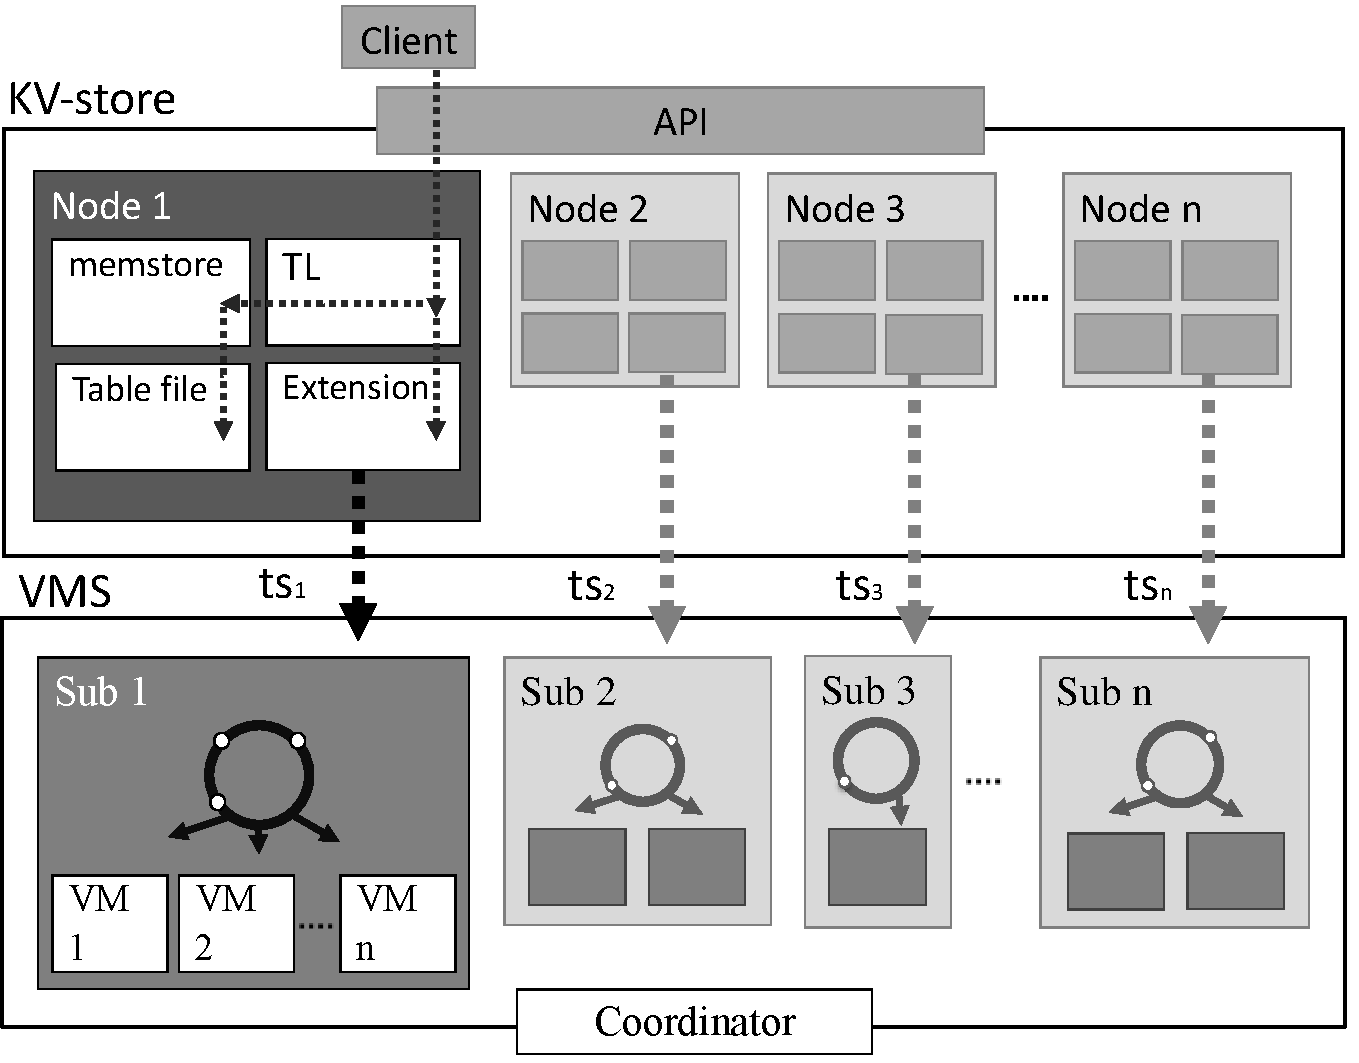
\includegraphics[width=\linewidth]{figures/SystemOverview}  
	\caption{System Overview} 
	\label{fig:system_overview} 
\end{figure} 





The View Maintenance System receives updates from the KV-store in form
of operation streams (see Figure~\ref{fig:system_overview}). Every node
of the KV-store produces a local transaction stream ($ts_1,..,ts_n$);every 
stream of operations is handled by a subsystem of the VMS. The subsystem 
parallizes view update computation: it distributes the updates to a
scalable number of view managers. A view manager actually applies the
update operation to the view table. First, it looks up the view tables 
 defined over the base, then it retrieves the corresponding view record, 
adds the delta to it, and writes back the result to the view.

We express view tables in the VMS with the help of relational algebra 
(e.g., we define a \texttt{SELECTION} as $S=\sigma_{c_1 < x}(A)$ over a 
base table $A$). Defining a view table over a base table is equivalent
to connection the output stream of base table operations with the input
stream of view table input operations. The VMS is also capable of 
defining view tables over view tables (e.g. we define a \texttt{PROJECTION}
view as $P=\pi_{c_1,c_2}(S)$). Thus,
we can concatenate multiple different view types; the VMS will update the
view chain subsequently. It will receive the base table update, apply the
update to the \texttt{SELECTION} view, and apply the result of the first
update to the \texttt{PROJECTION} view.